\section{Final Solution}
Our final AUC score of 0.90918 results from a complex pipeline from raw data to final score.
Every part of that pipe needs to be (sub-)optimal implemented by our team to get the best score at the end.
The first part ``feature design'' is the most important one and needs expertise, experience and of course a bit luck to capture all signals in the data.

We train 64 single models with 7 algorithms and 7 feature sets.

\begin{table*}[t]
\begin{center}
\begin{tabular}{lllll}
\label{tb:singleModels}
ID	& Model 				& Feature						& 5-CV		& Public Leaderboard \\ 
\hline
S1 	& xgb\_rf\_ko\_new\_feat 	& F2 + F3 + F6 + F7				& 0.906721	& 0.907765 \\
S2 	& ko\_v83			 	& F2 + F1 + F6 + F7 				& 0.906729	& 0.907525\\
S3 	& bag\_10\_xgb\_rf.xiv  	& F2 + F1 + F3 					& 0.905875 	& 0.906361 \\
S4 	& xgb\_rf.xvi			& F2 + F3 + F6					& 0.905543	& 0.905516 \\
S5 	& xgb\_rf.xix			& F2 + F1 + F3 + F5				& 0.905356	& - \\
S6	& rw\_sk\_xgb			& F2 + F1						& 0.905312	& - \\
S7	& xgb\_rf.xv			& F2 + F3						& 0.904935	& 0.905480 \\
S8	& xgb\_rw\_sk			& F2 + F1						& 0.904914	& - \\
S9	& mjahrer.feat.tam+rw+sk+tam2+sk2+azure.dae+nn	& F2 + F1 + F3 + F4 & 0.904235 & - \\
S10	& mjahrer.featmjahrer+Tam+RW+KoheiSong.nn & F2 + F1 + F3 + F4 & 0.903736 & - \\
S11	& mjahrer.featTam+RW+KoheiSong.dae+nn & F2 + F1 + F3 & 0.903669	& - \\
S12	& pred\_train\_sk\_feature\_ffm\_rw & F1 + F2 				& 0.903560	& 0.904411 \\
S13	& mjahrer.featTam+RW+KoheiSong.nn & F2 + F1 + F3 		& 0.903428	& - \\
S14	& xg\_400\_4\_0.05\_feature\_rw & F2 + F6				& 0.903385	& - \\
S15 	& kohei\_song			& F1							& 0.902918	& - \\
S16 	& xgb\_cv\_rw			& F2 						& 0.902287	& - \\
S17	& ffm\_cv\_rw			& F2							& 0.901983	& - \\
S18	& mjahrer.dae+nn.RWfeat	& F2							& 0.901846	& 0.902614 \\
S19	& mjahrer.featmjahrer+Tam+RW+KoheiSong.dae+krr & F2 + F1 + F3 + F4	& 0.901522	& - \\
S20 	& mjahrer.feat.tam+rw+sk+tam2+sk2+azure.BIN & F2 + F1 + F3 & 0.900982	& - \\
S21	& xg\_400\_4\_0.05\_feature\_sk	& F1					& 0.900906	& - \\
S22	& xgb\_rf.xiv			& F3							& 0.899239	& - \\
S23	& xgb\_rf.xiv			& F3							& 0.899167	& - \\
S24	& xgb\_rf.xiv			& F3							& 0.898969	& - \\
S25 	& xgb\_rf.xiv			& F3							& 0.898890	& - \\
S26 	& xgb.xiv				& F3							& 0.898749	& - \\
S27	& libfm\_100\_4\_0.002\_feature\_rw\_v2	& F2 + F6			& 0.898308	& - \\
S28  & xgl\_500\_0.5\_10\_10\_feature\_rw\_v2	& F2 + F6			& 0.897968	& - \\
S29	& xgb\_val.xiii			& F3							& 0.897912	& - \\
S30	& nn\_20\_16\_0.01\_feature\_rw\_v2	& F2 + F6			& 0.897143	& - \\
S31	& mb\_nn\_50\_20\_feat19	& F2 + F5					& 0.896748	& - \\
S32	& sm\_rw\_sk\_tam		& F2 + F1 + F3					& 0.896435 	& - \\
S33  & ffm\_30\_20\_0.01\_feature\_rw\_v2	& F2 + F6			& 0.896160	& - \\
S34  & xg\_400\_4\_0.05\_feature\_tam	& F3					& 0.895754	& - \\
S35	& ConfigAMLKRR		& F4							& 0.894524	& - \\
S36 	& gbm.xiii				& F3							& 0.893507	& - \\
S37	& xg\_600\_4\_0.05\_feature10	& F6						& 0.892364	& - \\
S38 	& xg\_600\_4\_0.05\_feature9	& F6						& 0.892253	& - \\
S39 	& ConfigAML			& F4							& 0.891217	& - \\
S40	& lr\_0.01\_feature\_tam	& F3							& 0.890580	& - \\
S41	& ConfigAMLCUDAPreModel	& F4						& 0.890565	& - \\
S42 	& ffm\_30\_20\_0.01\_feature\_tam	& F3					& 0.888418	& - \\
S43	& libfm\_100\_4\_0.002\_feature\_tam	& F3				& 0.888381	& - \\
S44	& rf.xiii				& F3							& 0.887583	& - \\
S45	& et\_1000\_20\_feature\_tam	& F3						& 0.887768	& - \\
S46 	& ffm\_30\_20\_0.01\_feature9	& F6						& 0.887116	& - \\
S47	& libfm\_100\_4\_0.002\_feature9	& F6					& 0.886866	& - \\
S48	& ConfigAML			& F4							& 0.886705	& - \\
S49	& nn\_20\_16\_0.01\_feature9	& F6						& 0.886109	& - \\
S50 	& xg\_400\_4\_0.05\_feature6	& F6						& 0.885184	& - \\
S51 	& xg\_400\_4\_0.05\_feature3	& F6						& 0.885124	& - \\
S52 	& ffm\_20\_20\_0.01\_feature6	& F6						& 0.885037	& - \\
S53	& ffm\_20\_20\_0.01\_feature3	& F6						& 0.884697	& - \\
S54 	& xg\_400\_4\_0.05\_feature\_mj	& F4					& 0.882441	& - \\
S55	& et\_1000\_20\_feature\_rw\_v2	& F2 + F6				& 0.881539	& - \\
S56	& libfm\_100\_8\_0.01\_feature6	& F6					& 0.880878	& - \\
S57	& libfm\_100\_8\_0.01\_feature3	& F6					& 0.880366	& - \\
S58	& nn\_20\_16\_0.005\_feature3	& F6						& 0.880219	& - \\
S59	& ConfigAMLKNN		& F4							& 0.877652	& - \\
S60	& nn\_20\_16\_0.005\_feature5	& F6						& 0.876905	& - \\
S61	& lr\_0.01\_feature\_mj		& F4						& 0.821332	& - \\
S62	& lr\_0.01\_feature9		& F6							& 0.804150	& - \\
S63	& lr\_0.01\_feature3		& F6							& 0.802138	& - \\
S64	& lr\_0.01\_feature6		& F6							& 0.800225	& - \\
\end{tabular}
\end{center}
\end{table*}

We trained 15 stage-I ensemble classifiers with different subsets of CV predictions of 64 single classifiers.

At KDD Cup 2015, GBM outperforms other algorithms.  Our top 8 single models as well as top 2 stage-1 ensemble models are trained with GBM.

We trained 2 stage-II ensemble classifiers with different subsets of CV predictions of 15 stage-I ensemble classifiers.

We trained a stage-III ensemble classifier with CV predictions of 5 classifiers: 1 stage-II ensemble, 3 stage-I ensemble, and 1 individual classifiers.

Performance improvement diminishes as we add more ensemble stages.  The stage-1 ensemble improves the CV AUC score by XXXX from 0.906721 to 0.907688.  The stage-2 ensemble improves the CV AUC score by XXXX to 0.907968.  The stage-3 ensemble improves the CV AUC score by XXXX to 0.908194.\\

We choose subsets of predictions from the previous stage for ensemble model training, 
\begin{figure*}[!ht]
  \caption{5-fold CV vs. public leaderboard AUC scores}
  \centering
    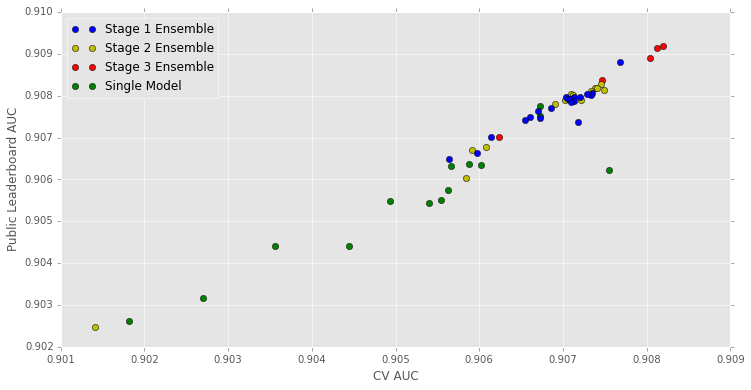
\includegraphics[width=0.5 \textwidth]{cv_lb}
\end{figure*}



\begin{table*}[t]
\begin{center}
\begin{tabular}{lllll}
\label{tb:ensembleModels}
ID	& Stage	& Model 				& 5-CV		& Public Leaderboard \\ \hline
E1	& III		& subBlend\_0712v2		& 0.908194 	& 0.909181 \\
E2	& II		& lr\_forward\_0.01\_esb.esb15v3 & 0.907968	& - \\
E3	& II		& xgl\_10\_0.01\_10\_10\_esb.esb11v6 & 0.907379 & 0.908187 \\
E4 	& I		& at.esb50v2+ko			& 0.907878	& - \\
E5	& I		& xg\_sk\_1800\_5\_0.004\_esb51\_rank & 0.907734 \\
E6 	& I		& lr\_forward\_0.01\_esb51\_rank\_norm & 0.907716	& - \\
E7	& I		& song\_train\_xgb\_esb58v5\_ko & 0.907668	& 0.908796 \\
E8	& I		& esb58v5+magic.dae+nn		& 0.907567	& - \\
E9	& I		& esb58v3.trn.final			& 0.907353	& 0.908060 \\
E10	& I		& trn.esb56.blend.at			& 0.907283	& 0.908043 \\
E11 	& I		& ConfigAMLCUDAPreModel	& 0.907076	& - \\
E12	& I		& xg\_sk\_1800\_5\_0.004\_esb56\_rank\_4 & 0.907036	& 0.907977 \\
E13 	& I		& esb55.dae+nn			& 0.906956	& - \\
E14	& I		& lr\_0.01\_esb51\_rank\_norm	& 0.906746	& - \\
E15 	& I		& nn						& 0.906714	& - \\
E16	& I		& xgb\_rf\_esb55.xix			& 0.906689	& - \\
E17	& I		& libfm					& 0.906537	& - \\
E18 	& I		& et\_esb58v5\_rank			& 0.906200	& - \\
\end{tabular}
\end{center}
\end{table*}

A linear combination of the 5 models from table \ref{tb:finalEnsemble} results in train AUC=0.908072 and accuracy=0.887334.
Which leads to 0.90910 public leaderboard score.
By adding 39 courseID correction factors train AUC=0.908194 and public score improved to 0.90918.

\begin{figure*}[!ht]
  \caption{End-to-end pipeline for the final solution}
  \centering
    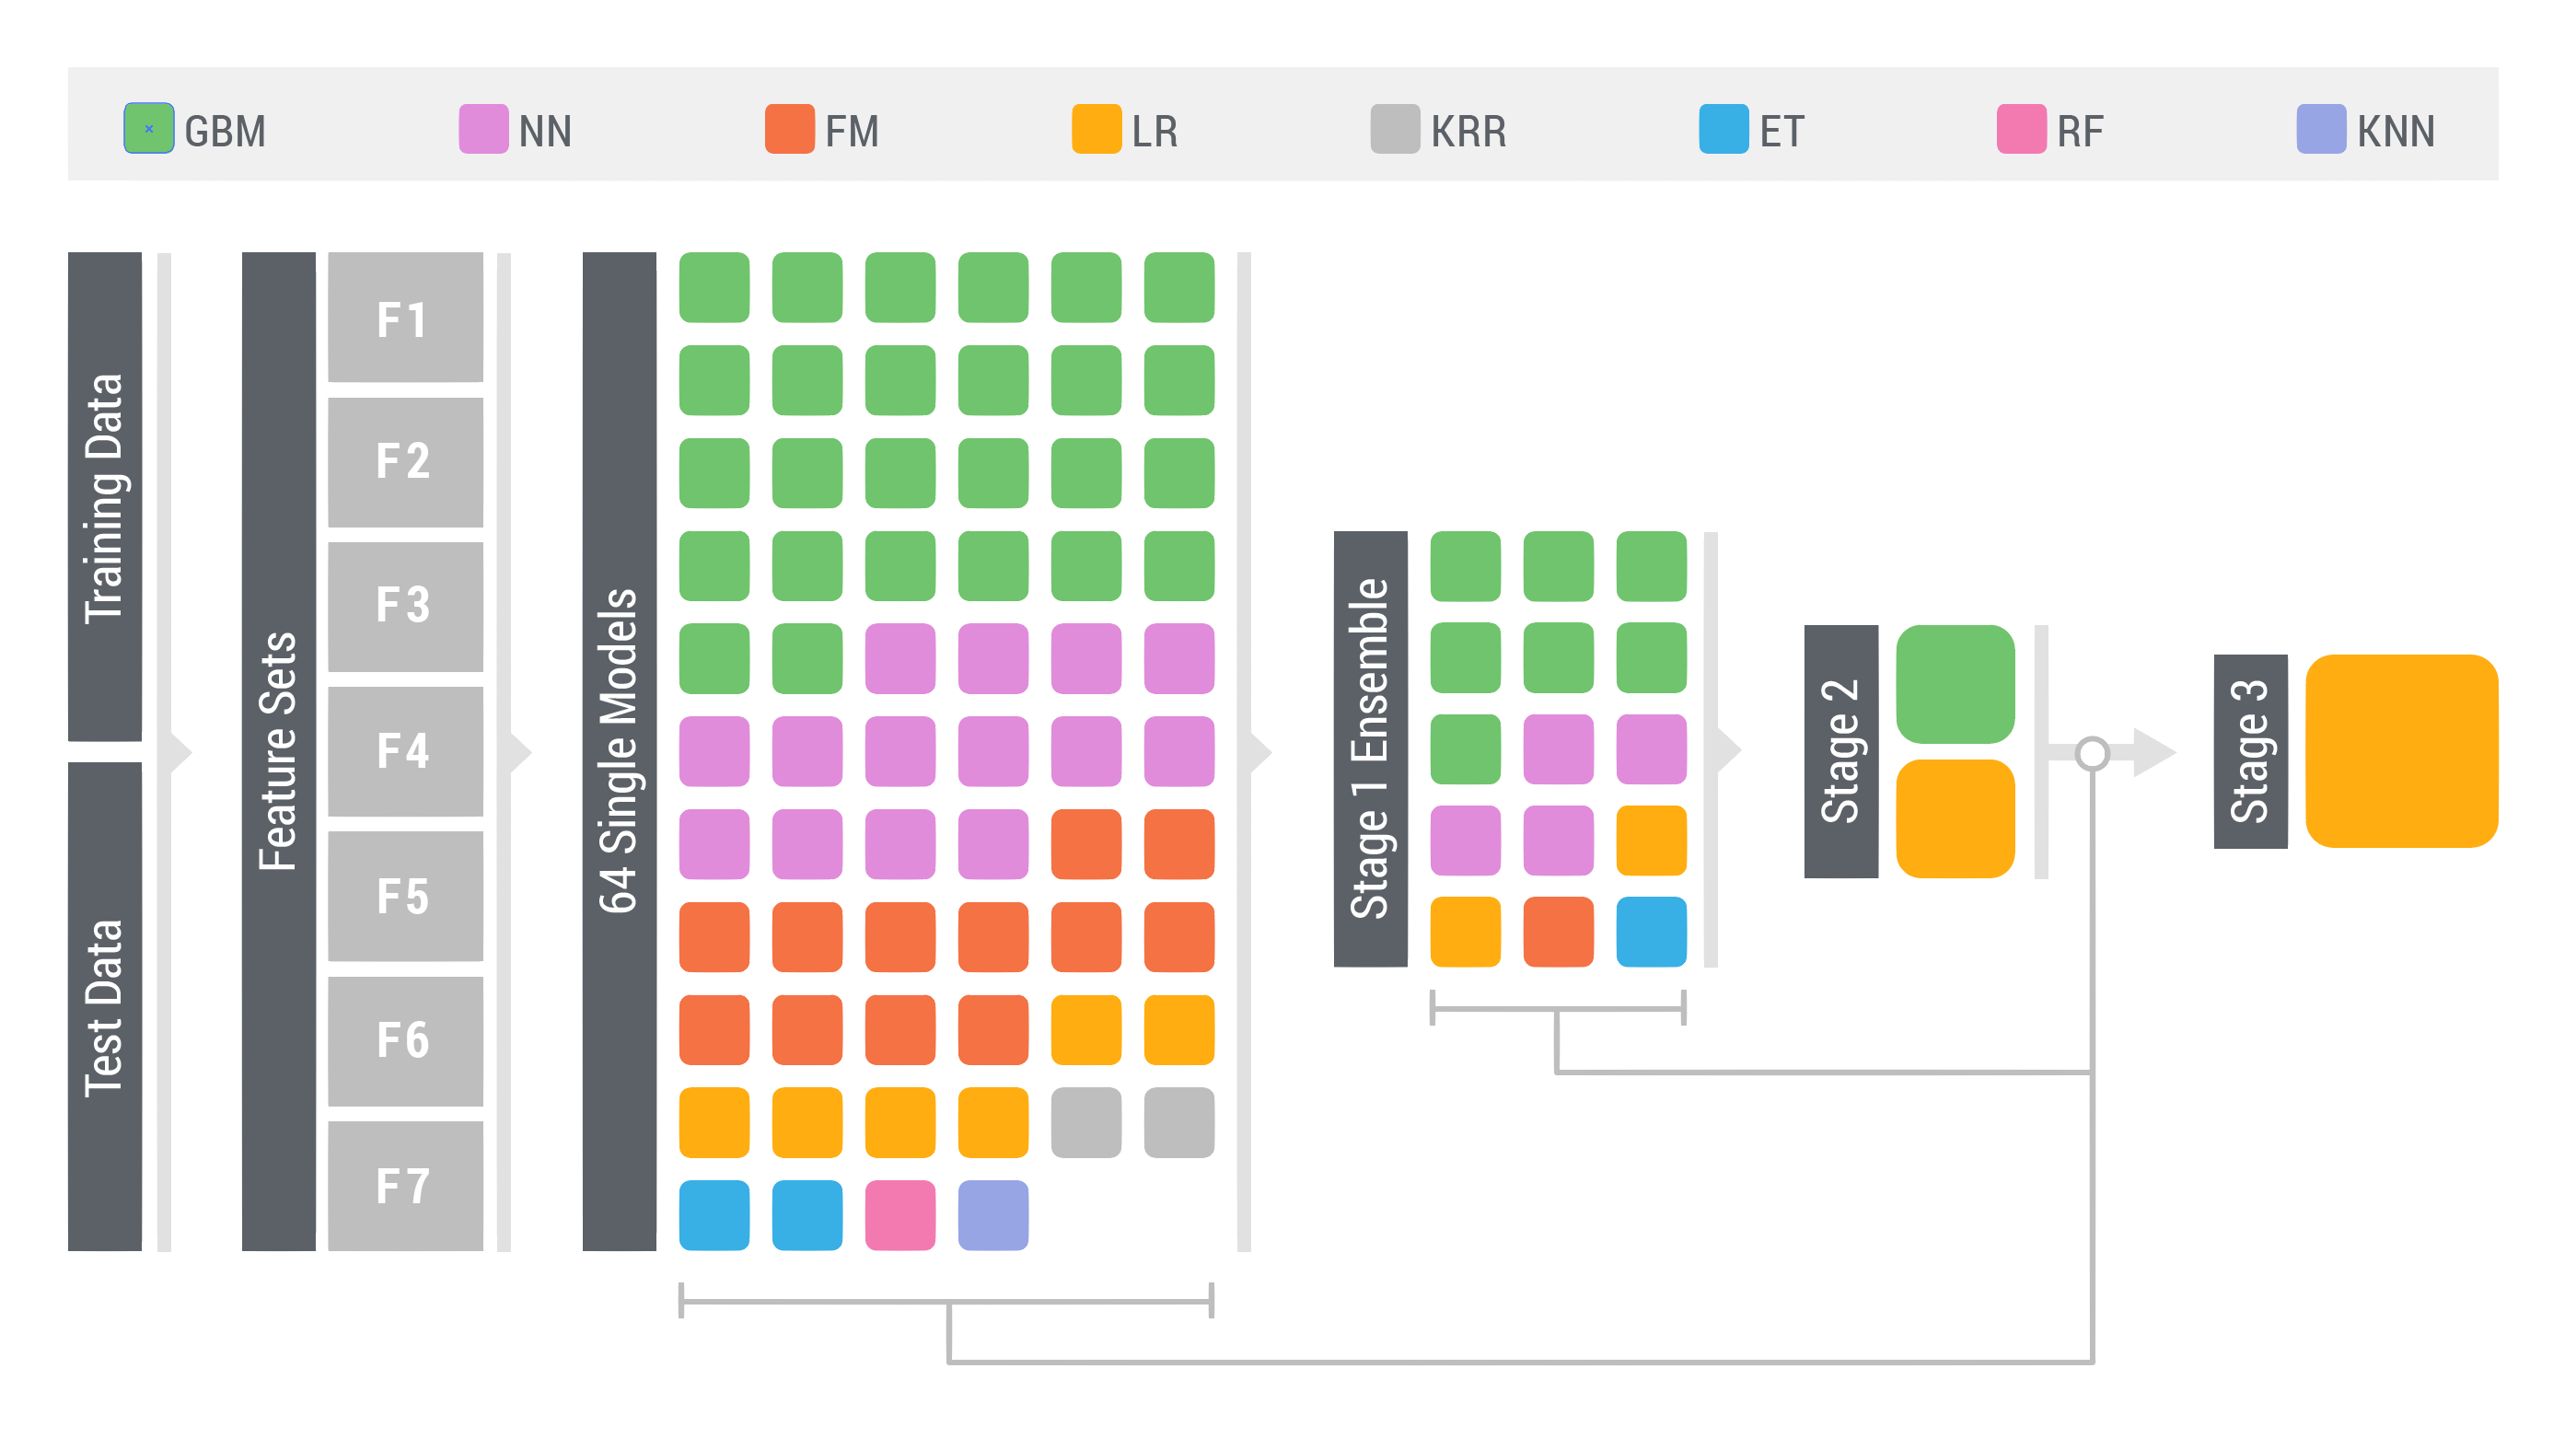
\includegraphics[width=1 \textwidth]{ensemble}
\end{figure*}

\begin{center}
\begin{tabular}{lllll}
\label{tb:finalEnsemble}
ID 	& Model 				& Type 	& 5-CV 		& Weight\\ \hline
S1 	& xgb\_rf.ko\_new\_feat 	& Single 	& 0.906721 	& 1.1703 \\
E4 	& at.esb50v2+ko 		& Stage I 	& 0.907878 	& 1.9626\\
E8 	& esb58v5+magic.dae+nn & Stage I & 0.907567	& 0.7871\\
E18	& et\_esb58v5\_rank		& Stage I	& 0.906207 	& 0.4580\\
E2	& lr\_forward\_0.01\_esb.esb15v3 & Stage II & 0.907968 & 1.6146\\
\end{tabular}
\end{center}

